\documentclass[a4paper]{article}
\usepackage{hyperxmp}
\usepackage{titling}
\usepackage[colorlinks,linkcolor=blue]{hyperref}
\usepackage{graphicx}
\usepackage{fancyhdr}
\usepackage{a4wide}
\usepackage{xspace}
\usepackage{lastpage}
\usepackage{ccicons}
%\usepackage{wrapfig}
%\usepackage{multicol}

\newcommand{\myhref}[2]{{\href{#1}{\textcolor{blue}{#2}}}}

\fancyhead[L]{\thetitle}
\fancyhead[R]{\it\thepage\ of \pageref{LastPage}}
\fancyfoot[C]{\centerline{\small \ccbysa\ \theauthor, 2013. This work is licensed under a \myhref{http://creativecommons.org/licenses/by-sa/3.0/}{Creative Commons Attribution-ShareAlike 3.0 Unported License.}}}
\pagestyle{fancy}

%% PDF meta-data
\hypersetup{%
pdftitle={Assigment 3 for the course on city design. A vision for your city.}
pdfauthor={Vitaly Repin},
pdfcopyright={This work is licensed under a Creative Commons Attribution-ShareAlike 3.0 Unported License},
pdfsubject={Designing City},
pdfkeywords={design,city,map}
pdflicenseurl={http://creativecommons.org/licenses/by-sa/3.0/},
pdfcaptionwriter={Vitaly Repin},
pdfcontactcity={Espoo},
pdfcontactcountry={Finland},
pdfcontactemail={vitaly.repin@gmail.com},
pdflang={en}
}

%% Author
\author{Vitaly Repin}
%% Title
\title{[Draft] A Vision For \emph{Greater Helsinki}: Bicycling Route Signage}

\date{December, 2013}

\begin{document}
\section{Executive summary}
I suggest to extend the existing system of the pointers for the bicyclists. The main idea is to add numbered bicycling routes to the bicycle signaling system.
It is inspired by the Bicycling Route Network of Switzerland.

Key elements of the proposal:

\begin{itemize}
\item Create a web site with regional bicycling routes (numbered)
\item Add pointers with the bicycle route numbers to the existing traffic signs
\item Connect the pointers signs with web site resources through QR codes (unique QR code drawn on every pointer)
\end{itemize}

Benefits:

\begin{itemize}
\item Promoting region as a bicycling paradise (touristic industry)
\item Promoting local places (shops, restaurants, hotels, museums etc) through the web site and QR-codes drawn on the pointers (geographically-targeted advertisements)
\item Moving the bicyclists away from the automobile roads (increasing road safety)
\end{itemize}

\section{Introduction}
Greater Helsinki is metropolitan area including smaller Capital Region urban kernel and commuter towns surrounding Helsinki, the capital of Finland.

These regions are located in the south of Finland, on the coast of the Gulf of Finland, which is part of the Baltic Sea. The smaller region includes Helsinki, Vantaa, Espoo, and Kauniainen and has a population of about one million. The Helsinki region is the largest urbanised area in the country, and is by far the most important economic, cultural, as well as scientific region of Finland.
Seven out of Finland's 17 universities and most of the headquarters of notable companies and governmental institutions are located in Greater Helsinki, as is Finland's main aviation hub,
Helsinki Airport, which is located in Vantaa~\cite{GHel}.

The region is bicyclist-friendly. It contains a lot of dedicated lanes for bicyclists.

\section{Current state}
\subsection{Web resources}
\begin{itemize}
\item \myhref{http://pk.reittiopas.fi/en/}{Helsinki Journey Planner} allows to plan bicycling route
\item \myhref{http://www.ulkoilukartta.fi/}{Outdoor recreation and cycling map}
\item \myhref{http://www.pyoraillensuomessa.fi/en/node/2}{National Cycling routes} are going through Greater Helsinki area
\end{itemize}

\subsection{Paper maps}
\myhref{http://www.ulkoilukartta.fi/}{Outdoor recreation and cycling map} is available for free in a lot of places in Greater Helsinki area.

\subsection{Traffic signs}
\begin{figure}[!h]
\centerline{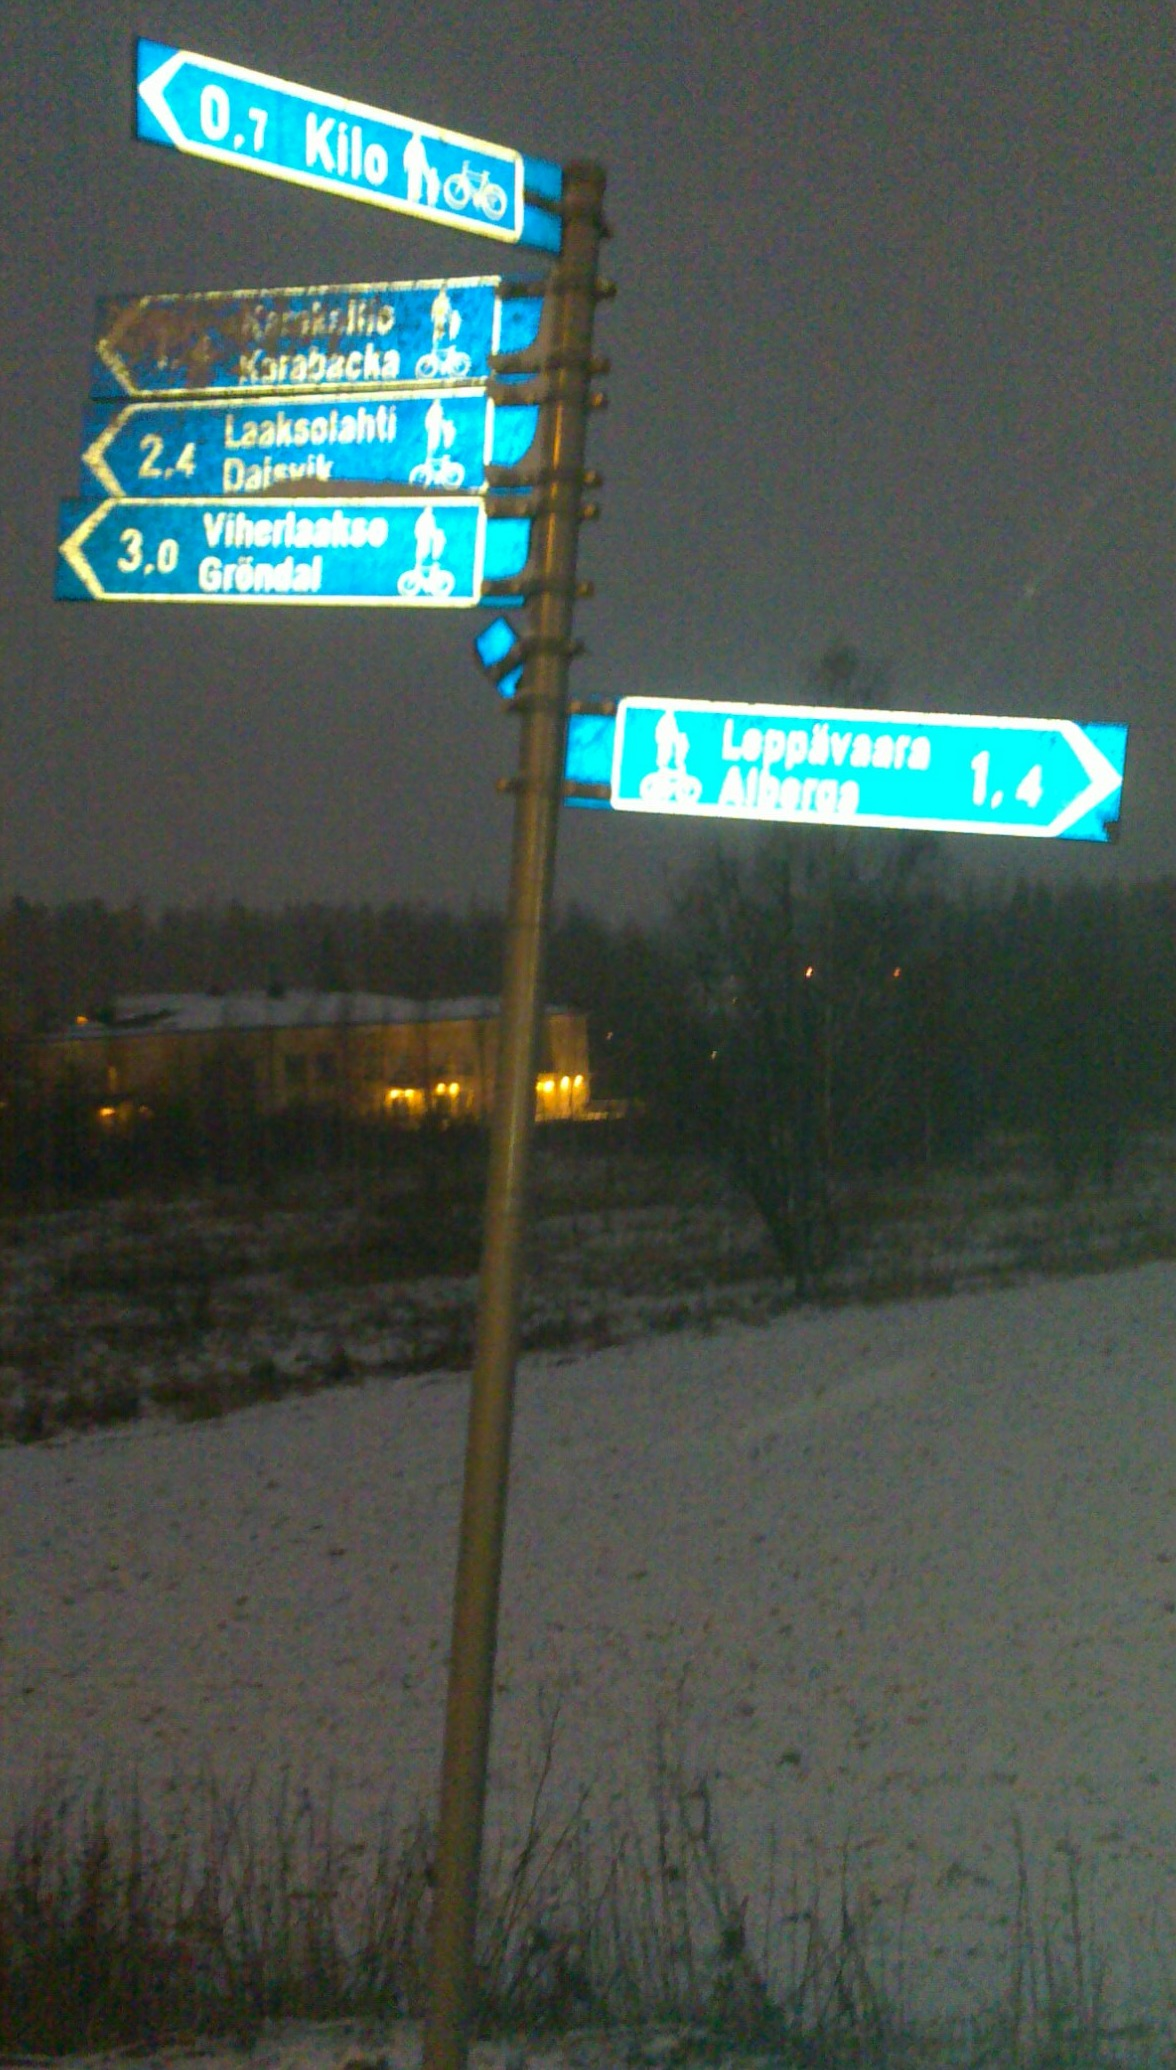
\includegraphics[keepaspectratio,height=6.5cm]{kilo}}
\caption{Current traffic signs for bicyclists}
\end{figure}

Currently the traffic signs for the bicyclists mention only the directions to the closest municipality/point of interest/etc. No data about the bicycling route exists.

\section{Proposed solution}
\begin{itemize}
\item Create a web site with regional bicycling routes. Every route should have its number.
\item Add the number of the routes to the traffic signs (see examples in the section~\ref{s:example}).
\item Add unique QR code with the hyperlink to the tourist web site to every new traffic sign installed. This link will contains the data about the closest point of interests (including
restaurants, hotels, museums etc)
\end{itemize}

Stakeholders:
\begin{itemize}
\item City planning departments
\item Tourist industry association
\item Bicycling clubs
\end{itemize}

\section{Success stories\label{s:example}}
Switzerland is very famous for its bicycling network.  They have the network of bicycling routes covering the whole country, web sites describing the routes and
traffic signs with the numbers of the routes.

\begin{figure}[!h]
\centerline{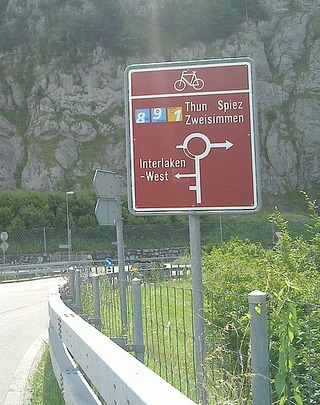
\includegraphics[keepaspectratio,height=6.5cm]{thun1}}
\caption{Switzerland: Bicycle route signs. Complex case}
\end{figure}

\begin{figure}[!h]
\centerline{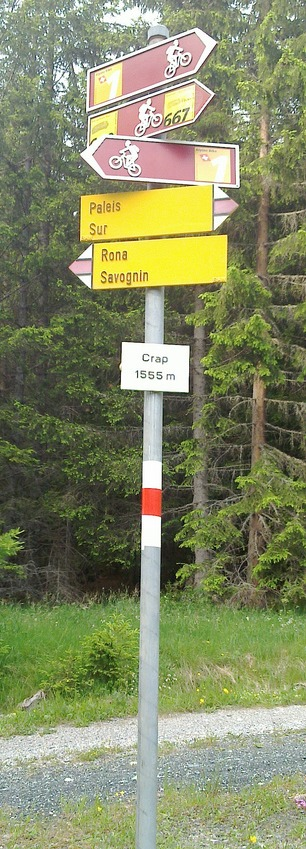
\includegraphics[keepaspectratio,height=6.5cm]{swiss1}}
\caption{Switzerland: Bicycle route signs. Simple case}
\end{figure}
\newpage

\begin{thebibliography}{9}
\bibitem{GHel} \myhref{http://en.wikipedia.org/wiki/Greater_Helsinki}{Greater Helsinki. Wikipedia article.}
\end{thebibliography}
\end{document}
